\documentclass[a4paper]{article}

% Global layout
\usepackage{fancyhdr, graphicx, hyperref, indentfirst, lastpage, setspace}
\usepackage[margin=40mm]{geometry}

% Encoding
\usepackage[utf8]{vntex, inputenc} % vntex first to avoid Vietnamese auto captions
\usepackage{amsmath, amssymb, gensymb}

% Better table
\usepackage{array, booktabs, multicol, multirow, siunitx}

% Code space
\usepackage[dvipsnames]{xcolor}
\usepackage{tikz}
\usepackage[framemethod=tikz]{mdframed}
\usepackage{minted} % needs --shell-escape flag and Pygments

% Extra
\usepackage{caption, float}

% Page setup
% \allowdisplaybreaks{} % to have page breaks inside align* environment
\hypersetup{urlcolor=blue,linkcolor=black,citecolor=red,colorlinks=true}
\usemintedstyle{emacs}
\numberwithin{equation}{section}
\renewcommand{\arraystretch}{1.2} % space between table rows

% Custom enumerating
\usepackage{enumitem}
\newlist{steps}{enumerate}{1}
\setlist[steps, 1]{label = Step \arabic*:}
% Global style setup
\makeatletter % change font size for not having underfull hbox
\renewcommand\Huge{\@setfontsize\Huge{22pt}{18}}
\makeatother

\AtBeginDocument{\renewcommand*\contentsname{Contents}}
\AtBeginDocument{\renewcommand*\refname{References}}
\setlength{\headheight}{40pt}
\pagestyle{fancy}
\fancyhead{} % clear all header fields
\fancyhead[L]{
  \begin{tabular}{rl}
    \begin{picture}(25,15)(0,0)
    \put(0,-8){
\includegraphics[width=8mm, height=8mm]{hcmut.png}}
    \end{picture}
    \begin{tabular}{l}
      \textbf{\bf \ttfamily University of Technology, Ho Chi Minh City}\\
      \textbf{\bf \ttfamily Faculty of Computer Science and Engineering}
    \end{tabular}
  \end{tabular}
}
\fancyhead[R]{
	\begin{tabular}{l}
		\tiny \bf \\
		\tiny \bf
	\end{tabular}  }
\fancyfoot{} % clear all footer fields
\fancyfoot[L]{\scriptsize \ttfamily Assignment for Operating System --- Academic year 2020--2021}
\fancyfoot[R]{\scriptsize \ttfamily Page {\thepage}/\pageref{LastPage}}
\renewcommand{\headrulewidth}{0.3pt}
\renewcommand{\footrulewidth}{0.3pt}

\everymath{\color{blue}}

\newcommand*\mean[1]{\bar{#1}}

\begin{document}

\begin{titlepage}
  \begin{center}
    VIETNAM NATIONAL UNIVERSITY, HO CHI MINH CITY \\
    UNIVERSITY OF TECHNOLOGY \\
    FACULTY OF COMPUTER SCIENCE AND ENGINEERING
  \end{center}

  \vspace{1cm}

  \begin{figure}[H]
    \centering
    
\includegraphics[scale = 0.5]{hcmut.png}
  \end{figure}

  \vspace{1cm}

  \begin{center}
    \begin{tabular}{c}
      \textbf{\Large OPERATING SYSTEM (CO2018)}                     \\
      {}                                                            \\
      \midrule                                                      \\
      \textbf{\Large Assignment (Semester 202, Duration: 03 weeks)} \\
      {}                                                            \\
      \textbf{\Huge Simple Operating System}                        \\
      {}                                                            \\
      \bottomrule
    \end{tabular}
  \end{center}

  \vspace{3cm}

  \begin{table}[h]
    \begin{tabular}{lll}
      \hspace{1cm} Advisor:  & Ms.\ Lê Thanh Vân                                   \\
      \hspace{1cm} Students: &                                                     \\
                             & Nguyễn Hoàng (CC02, \textbf{Team leader}) & 1952255 \\
                             & Đỗ Đăng Khoa (CC02)                       & 1952295 \\
                             & Lê Minh Đăng (CC02)                       & 1952041 \\
    \end{tabular}
  \end{table}

  \begin{center}
    {\footnotesize HO CHI MINH CITY, MAY 2021}
  \end{center}
\end{titlepage}


%\thispagestyle{empty}

\newpage
\tableofcontents

\newpage
%%%%%%%%%%%%%%%%%%%%%%%%%%%%%%%%%
\section{Scheduling}
\subsection{Priority feedback queue versus the world}
The Priority Feedback Queue (PFQ) takes after some designing concept from the Multilevel Feedback Queue, i.e.\ using more than one queue to schedule process.
The \textbf{time slot} --- based on the Round Robins with Quantum time --- is used to schedule the process.

The PFQ uses two queues with the following functions
\begin{itemize}
  \item \mintinline{C}{ready_queue}: Contains all the processes and their priority to be executed.
        It will run before \mintinline{C}{run_queue}.
        When the CPU switches to a process, the dispatcher will take one from \mintinline{C}{read_queue}.

  \item \mintinline{C}{run_queue}: Contains the processes which have been executed but have yet to finish.
        All the processes from this queue get to be executed only if the \mintinline{C}{ready_queue} is empty.

  \item The procedure that we use to implement \mintinline{C}{enqueue()} operation will based on the concept of basic priority queue
\end{itemize}

\subsection{Advantages of Priority feedback queue}
The priority feedback queue holds several advantages over other scheduling algorithms.

First and foremost, it implements a mechanism where the relative importance of each process can be defined, meaning that we can have certain processes run before the others.

Let's talk about the advantages of PFQ first:
\begin{itemize}
  \item PFQ will ensure that all processes will be executed.
        In other words, it solves the starvation problem by respecting the order of the processes, ensuring all processes are executed.
  \item The algorithm uses a time slot like the Round-Robin algorithm with a quantum time for each process, thus allowing us to tune the quantum time to minimize average response and turnaround time.
\end{itemize}

Other scheduling algorithms pose downsides in comparison with priority feedback queue as follows
\begin{itemize}
  \item First come first served
        Here, the earlier process will be allocated the CPU first, other processes have to wait until the current process has finished its execution.
        For example, suppose the first process has a very long burst time, and other processes have less burst time, then the later processes will have to wait longer, this will result in more average waiting time, also known as Convey effect.

  \item Shortest job first, Shortest runtime first
        Here, the process with shorter burst time is executed first, meaning that processes with long burst time will be pushed further back in the queue, and potentially never executed.
        This is known as starvation.
        In the case that any process always finishes before another one arrives, SJF/SRTF becomes FCFS.\

  \item Round Robin
        The CPU cycles through all processes in the queue for the amount of time designated by the quantum time or if the process finishes before the quantum time runs out.
        Choosing an optimal quantum is hard: too short and the overhead for context switching outweighs the runtime, too long and it becomes FCFS.\

  \item Multilevel
        This is a combination of multiple kinds of scheduling algorithms.
        Processes at the lowest level might suffer from starvation if the implementation is not thoroughly considered.
\end{itemize}

\subsection{Gantt chart of this assignment's scheduler}
Here, we will draw 2 Gantt diagrams that represent the workflow covering the following tests: \mintinline{C}{sched_0} and \mintinline{C}{sched_1}.
The implemented scheduling algorithm is the aforementioned priority feedback queue in the Round-Robin style, with a time quantum of 2 time units for both tests.

\begin{itemize}
  \item \mintinline{C}{sched_0}
\end{itemize}

The processes of \mintinline{C}{sched_0} are summarized in the table below:

\begin{table}[H]
  \centering
  \begin{tabular}{cccc}
    \toprule
    Process & Arrival time & Burst Time & Priority \\
    \midrule
    s0      & 0            & 15         & 12       \\
    s1      & 4            & 7          & 20       \\
    \bottomrule
  \end{tabular}
\end{table}

We obtain the following Gantt diagram that shows how the CPU chooses which process to run, assuming that the loader routine runs ahead of the CPU routine.

\begin{figure}[H]
  \centering
  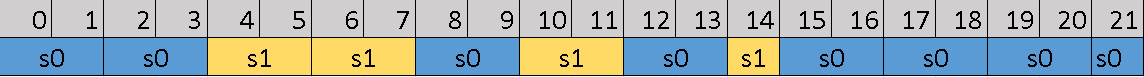
\includegraphics[width=0.9\textwidth]{sched_0.png}
  \caption{Gantt diagram of \mintinline{C}{sched_0}}
\end{figure}

The simulated OS should print something akin to this proposed schedule.
Here is what \mintinline{C}{sched_0} returned.
Notice that the process with PID 1 is s0 and the one with PID 2 is s1.

\begin{mdframed}[leftline=false,rightline=false,backgroundcolor=teal!10,nobreak=false]
  \begin{minted}[linenos,breaklines,breaksymbolleft=,obeytabs=true,tabsize=2]{text}
------ SCHEDULING TEST 0 -------------------------------------------
./os sched_0
Time slot   0
        Loaded a process at input/proc/s0, PID: 1
Time slot   1
        CPU 0: Dispatched process  1
Time slot   2
Time slot   3
        CPU 0: Put process  1 to run queue
        CPU 0: Dispatched process  1
Time slot   4
        Loaded a process at input/proc/s1, PID: 2
Time slot   5
        CPU 0: Put process  1 to run queue
        CPU 0: Dispatched process  2
Time slot   6
Time slot   7
        CPU 0: Put process  2 to run queue
        CPU 0: Dispatched process  2
Time slot   8
Time slot   9
        CPU 0: Put process  2 to run queue
        CPU 0: Dispatched process  1
Time slot  10
Time slot  11
        CPU 0: Put process  1 to run queue
        CPU 0: Dispatched process  2
Time slot  12
Time slot  13
        CPU 0: Put process  2 to run queue
        CPU 0: Dispatched process  1
Time slot  14
Time slot  15
        CPU 0: Put process  1 to run queue
        CPU 0: Dispatched process  2
Time slot  16
        CPU 0: Processed  2 has finished
        CPU 0: Dispatched process  1
Time slot  17
Time slot  18
        CPU 0: Put process  1 to run queue
        CPU 0: Dispatched process  1
Time slot  19
Time slot  20
        CPU 0: Put process  1 to run queue
        CPU 0: Dispatched process  1
Time slot  21
Time slot  22
        CPU 0: Put process  1 to run queue
        CPU 0: Dispatched process  1
Time slot  23
        CPU 0: Processed  1 has finished
        CPU 0 stopped

MEMORY CONTENT:
NOTE: Read file output/sched_0 to verify your result
  \end{minted}
\end{mdframed}

As we can see, after a process is loaded, it is not dispatched immediately.
This can be attributed to the 2 threads \mintinline{C}{loader_routine} and \mintinline{C}{cpu_routine} not starting in any given order.
The overall result should still resemble the hypothesized schedule.

\begin{itemize}
  \item \textbf{\mintinline{C}{sched_1}}
\end{itemize}

Similarly, the processes of \mintinline{C}{sched_1} are summarized in the table below:
\begin{table}[H]
  \centering
  \begin{tabular}{cccc}
    \toprule
    Process & Arrival time & Burst Time & Priority \\
    \midrule
    s0      & 0            & 15         & 12       \\
    s1      & 4            & 7          & 20       \\
    s2      & 6            & 12         & 20       \\
    s3      & 7            & 11         & 7        \\
    \bottomrule
  \end{tabular}
\end{table}

We expect the processes to be run as follows
\begin{figure}[H]
  \centering
  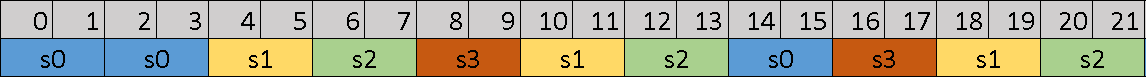
\includegraphics[width=0.9\textwidth]{sched_1a.png}

  \medskip
  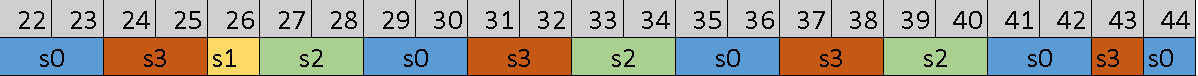
\includegraphics[width=0.9\textwidth]{sched_1b.png}
  \caption{Gantt diagram of \mintinline{C}{sched_1}}
\end{figure}

Here is how the simulated OS executed.
Note that the process with PID 1 is s0, the one with PID 2 is s1, the one with PID 3 is s2 and the remaining one is s4.

\begin{mdframed}[leftline=false,rightline=false,backgroundcolor=teal!10,nobreak=false]
  \begin{minted}[linenos=false,breaklines,breaksymbolleft=,obeytabs=true,tabsize=2]{text}
NOTE: Read file output/sched_0 to verify your result
------ SCHEDULING TEST 1 -------------------------------------------
./os sched_1
Time slot   0
        Loaded a process at input/proc/s0, PID: 1
Time slot   1
        CPU 0: Dispatched process  1
Time slot   2
Time slot   3
        CPU 0: Put process  1 to run queue
        CPU 0: Dispatched process  1
Time slot   4
        Loaded a process at input/proc/s1, PID: 2
Time slot   5
        CPU 0: Put process  1 to run queue
        CPU 0: Dispatched process  2
Time slot   6
        Loaded a process at input/proc/s2, PID: 3
Time slot   7
        CPU 0: Put process  2 to run queue
        CPU 0: Dispatched process  3
        Loaded a process at input/proc/s3, PID: 4
Time slot   8
Time slot   9
        CPU 0: Put process  3 to run queue
        CPU 0: Dispatched process  4
Time slot  10
Time slot  11
        CPU 0: Put process  4 to run queue
        CPU 0: Dispatched process  2
Time slot  12
Time slot  13
        CPU 0: Put process  2 to run queue
        CPU 0: Dispatched process  3
Time slot  14
Time slot  15
        CPU 0: Put process  3 to run queue
        CPU 0: Dispatched process  1
Time slot  16
Time slot  17
        CPU 0: Put process  1 to run queue
        CPU 0: Dispatched process  4
Time slot  18
Time slot  19
        CPU 0: Put process  4 to run queue
        CPU 0: Dispatched process  2
Time slot  20
Time slot  21
        CPU 0: Put process  2 to run queue
        CPU 0: Dispatched process  3
Time slot  22
Time slot  23
        CPU 0: Put process  3 to run queue
        CPU 0: Dispatched process  1
Time slot  24
Time slot  25
        CPU 0: Put process  1 to run queue
        CPU 0: Dispatched process  4
Time slot  26
Time slot  27
        CPU 0: Put process  4 to run queue
        CPU 0: Dispatched process  2
Time slot  28
        CPU 0: Processed  2 has finished
        CPU 0: Dispatched process  3
Time slot  29
Time slot  30
        CPU 0: Put process  3 to run queue
        CPU 0: Dispatched process  1
Time slot  31
Time slot  32
        CPU 0: Put process  1 to run queue
        CPU 0: Dispatched process  4
Time slot  33
Time slot  34
        CPU 0: Put process  4 to run queue
        CPU 0: Dispatched process  3
Time slot  35
Time slot  36
        CPU 0: Put process  3 to run queue
        CPU 0: Dispatched process  1
Time slot  37
Time slot  38
        CPU 0: Put process  1 to run queue
        CPU 0: Dispatched process  4
Time slot  39
Time slot  40
        CPU 0: Put process  4 to run queue
        CPU 0: Dispatched process  3
Time slot  41
Time slot  42
        CPU 0: Processed  3 has finished
        CPU 0: Dispatched process  1
Time slot  43
Time slot  44
        CPU 0: Put process  1 to run queue
        CPU 0: Dispatched process  4
Time slot  45
        CPU 0: Processed  4 has finished
        CPU 0: Dispatched process  1
Time slot  46
        CPU 0: Processed  1 has finished
        CPU 0 stopped

MEMORY CONTENT:
NOTE: Read file output/sched_1 to verify your result
  \end{minted}
\end{mdframed}

Once again, we can see that there are some minor differences between the observed and expected result.
Aside from that, the observed result should still represent the overall structure and scheduling order of the expected result.

\subsection{Code implementation for Scheduler:}
\subsubsection{queue.c}
We need to implement 2 functions, \mintinline{C}{enqueue()} and \mintinline{C}{dequeue()}.

\mintinline{C}{enqueue()} adds a new process to a specified queue.
While it is implemented using array, we will treat it as a queue, putting the processes with higher priority (smaller priority index) near the head of the queue.
\begin{mdframed}[leftline=false,rightline=false,backgroundcolor=magenta!10,nobreak=false]
  \begin{minted}[linenos=true,breaklines,breaksymbolleft=,obeytabs=true,tabsize=2]{C}
void enqueue(struct queue_t *q, struct pcb_t *proc)
{
  /* Put a new process to queue [q] */

  if (empty(q))
  {
    q->proc[0] = proc;
    (q->size) = 1;
    return;
  }

  if (full(q))
  {
    printf("Queue overflow");
    exit(1);
  }

  for (int i = q->size; i > 0; i -= 1)
  {
    if (q->proc[i - 1]->priority <= proc->priority)
    {
      q->proc[i] = proc;
      i = -1;
    }
    else
      q->proc[i] = q->proc[i - 1];

    if (i == 1)
      q->proc[0] = proc;
  }

  (q->size) += 1;
  return;
}
  \end{minted}
\end{mdframed}

About \mintinline{C}{dequeue()}, we just pop the head of the queue and move everything up afterwards.
In this assignment, elements are processes.
\begin{mdframed}[leftline=false,rightline=false,backgroundcolor=magenta!10,nobreak=false]
  \begin{minted}[linenos=true,breaklines,breaksymbolleft=,obeytabs=true]{C}
struct pcb_t *dequeue(struct queue_t *q)
{
  /*
   * Return a pcb whose priority is the highest
   * in the queue [q] and remember to remove it from q
   */

  if (q->size <= 0)
    return NULL;

  if (q->size >= MAX_QUEUE_SIZE) // * As if this will ever happen
    ;

  struct pcb_t *result = q->proc[0];

  for (int i = 0; i < q->size; i += 1)
    q->proc[i] = q->proc[i + 1];

  q->size -= 1;
  q->proc[q->size] = NULL;
  return result;
}
  \end{minted}
\end{mdframed}

\subsubsection{sched.c}
In sched.c, we need to implement the \mintinline{C}{get_proc()} method.
\mintinline{C}{get_proc()} will dequeue a process from the \mintinline{C}{ready_queue}.
If there is no process in the \mintinline{C}{ready_queue}, it will check the \mintinline{C}{run_queue} and push all the processes there.
\begin{mdframed}[leftline=false,rightline=false,backgroundcolor=magenta!10,nobreak=false]
  \begin{minted}[linenos=true,breaklines,breaksymbolleft=,obeytabs=true]{C}
struct pcb_t *get_proc(void)
{
  struct pcb_t *proc = NULL;
  /*
    * Get a process from [ready_queue]. If ready queue
    * is empty, push all processes in [run_queue] back to
    * [ready_queue] and return the highest priority one.
    * Remember to use lock to protect the queue.
    */

  pthread_mutex_lock(&queue_lock);

  if (empty(&ready_queue))
    while (!empty(&run_queue))
      enqueue(&ready_queue, dequeue(&run_queue));

  proc = dequeue(&ready_queue);

  pthread_mutex_unlock(&queue_lock);

  return proc;
}
  \end{minted}
\end{mdframed}

\newpage
\section{Memory Management}
\subsection{Advantage and disadvantage of segmentation with paging}
Segmentation with paging is a combination of both Segmentation and Paging techniques, where the main memory is divided into many segments with varying sizes and each segment houses a page table that further maps to many pages corresponding to frames in physical storage.

Upon a translation request is received, the Memory Management Unit will infer the position of the requested page from the virtual address by extracting the relevant bits, treating them as the indices to look for in the segment table and subsequently, the page table in said segment.

Compared to Segmentation or Paging alone, Segmentation with Paging introduces a wide range of advantages but also contributes a fair bit to the disadvantageous side.

\begin{itemize}
  \item \textbf{Advantages:}
        \begin{itemize}
          \item The page table size is reduced as pages are present only for data of segments, hence reducing the memory requirements.
          \item Segmentation with Paging reduces external fragmentation.
        \end{itemize}
  \item \textbf{Disadvantages:}
        \begin{itemize}
          \item It is much more complex, making it harder to implement and increasing the translation and memory access time.
          \item Memory is still vulnerable to internal fragmentation.
        \end{itemize}
\end{itemize}

\subsection{The memory after each allocation and deallocation call}
We will be modifying our program, namely the source file mem.c to call \mintinline{C}{dump()} right before \mintinline{C}{alloc_mem()} and \mintinline{C}{free_mem()} end.
The tests we will be using are \mintinline{C}{mem_0} and \mintinline{C}{mem_1}.

\begin{itemize}
  \item \textbf{\mintinline{C}{mem_0}}
\end{itemize}

\begin{mdframed}[leftline=false,rightline=false,backgroundcolor=teal!10,nobreak=false]
  \begin{minted}[linenos=false,breaklines,breaksymbolleft=,obeytabs=true,tabsize=2]{text}
------ MEMORY MANAGEMENT TEST 0 ------------------------------------
./mem input/proc/m0
Dumping memory content: #after alloc 13535 0
000: 00000-003ff - PID: 01 (idx 000, nxt: 001)
001: 00400-007ff - PID: 01 (idx 001, nxt: 002)
002: 00800-00bff - PID: 01 (idx 002, nxt: 003)
003: 00c00-00fff - PID: 01 (idx 003, nxt: 004)
004: 01000-013ff - PID: 01 (idx 004, nxt: 005)
005: 01400-017ff - PID: 01 (idx 005, nxt: 006)
006: 01800-01bff - PID: 01 (idx 006, nxt: 007)
007: 01c00-01fff - PID: 01 (idx 007, nxt: 008)
008: 02000-023ff - PID: 01 (idx 008, nxt: 009)
009: 02400-027ff - PID: 01 (idx 009, nxt: 010)
010: 02800-02bff - PID: 01 (idx 010, nxt: 011)
011: 02c00-02fff - PID: 01 (idx 011, nxt: 012)
012: 03000-033ff - PID: 01 (idx 012, nxt: 013)
013: 03400-037ff - PID: 01 (idx 013, nxt: -01)
Dumping memory content: #after alloc 1568 1
000: 00000-003ff - PID: 01 (idx 000, nxt: 001)
001: 00400-007ff - PID: 01 (idx 001, nxt: 002)
002: 00800-00bff - PID: 01 (idx 002, nxt: 003)
003: 00c00-00fff - PID: 01 (idx 003, nxt: 004)
004: 01000-013ff - PID: 01 (idx 004, nxt: 005)
005: 01400-017ff - PID: 01 (idx 005, nxt: 006)
006: 01800-01bff - PID: 01 (idx 006, nxt: 007)
007: 01c00-01fff - PID: 01 (idx 007, nxt: 008)
008: 02000-023ff - PID: 01 (idx 008, nxt: 009)
009: 02400-027ff - PID: 01 (idx 009, nxt: 010)
010: 02800-02bff - PID: 01 (idx 010, nxt: 011)
011: 02c00-02fff - PID: 01 (idx 011, nxt: 012)
012: 03000-033ff - PID: 01 (idx 012, nxt: 013)
013: 03400-037ff - PID: 01 (idx 013, nxt: -01)
014: 03800-03bff - PID: 01 (idx 000, nxt: 015)
015: 03c00-03fff - PID: 01 (idx 001, nxt: -01)
Dumping memory content: #after free 0
014: 03800-03bff - PID: 01 (idx 000, nxt: 015)
015: 03c00-03fff - PID: 01 (idx 001, nxt: -01)
Dumping memory content: #after alloc 1386 2
000: 00000-003ff - PID: 01 (idx 000, nxt: 001)
001: 00400-007ff - PID: 01 (idx 001, nxt: -01)
014: 03800-03bff - PID: 01 (idx 000, nxt: 015)
015: 03c00-03fff - PID: 01 (idx 001, nxt: -01)
Dumping memory content: #after alloc 4564 4
000: 00000-003ff - PID: 01 (idx 000, nxt: 001)
001: 00400-007ff - PID: 01 (idx 001, nxt: -01)
002: 00800-00bff - PID: 01 (idx 000, nxt: 003)
003: 00c00-00fff - PID: 01 (idx 001, nxt: 004)
004: 01000-013ff - PID: 01 (idx 002, nxt: 005)
005: 01400-017ff - PID: 01 (idx 003, nxt: 006)
006: 01800-01bff - PID: 01 (idx 004, nxt: -01)
014: 03800-03bff - PID: 01 (idx 000, nxt: 015)
015: 03c00-03fff - PID: 01 (idx 001, nxt: -01)
Dumping memory content: #final result
000: 00000-003ff - PID: 01 (idx 000, nxt: 001)
        003e8: 15
001: 00400-007ff - PID: 01 (idx 001, nxt: -01)
002: 00800-00bff - PID: 01 (idx 000, nxt: 003)
003: 00c00-00fff - PID: 01 (idx 001, nxt: 004)
004: 01000-013ff - PID: 01 (idx 002, nxt: 005)
005: 01400-017ff - PID: 01 (idx 003, nxt: 006)
006: 01800-01bff - PID: 01 (idx 004, nxt: -01)
014: 03800-03bff - PID: 01 (idx 000, nxt: 015)
        03814: 66
015: 03c00-03fff - PID: 01 (idx 001, nxt: -01)
NOTE: Read file output/m0 to verify your result
  \end{minted}
\end{mdframed}

\begin{itemize}
  \item \textbf{\mintinline{C}{mem_1}}
\end{itemize}

\begin{mdframed}[leftline=false,rightline=false,backgroundcolor=teal!10,nobreak=false]
  \begin{minted}[linenos=false,breaklines,breaksymbolleft=,obeytabs=true,tabsize=2]{text}
------ MEMORY MANAGEMENT TEST 1 ------------------------------------
./mem input/proc/m1
Dumping memory content: #after alloc 13535 0
000: 00000-003ff - PID: 01 (idx 000, nxt: 001)
001: 00400-007ff - PID: 01 (idx 001, nxt: 002)
002: 00800-00bff - PID: 01 (idx 002, nxt: 003)
003: 00c00-00fff - PID: 01 (idx 003, nxt: 004)
004: 01000-013ff - PID: 01 (idx 004, nxt: 005)
005: 01400-017ff - PID: 01 (idx 005, nxt: 006)
006: 01800-01bff - PID: 01 (idx 006, nxt: 007)
007: 01c00-01fff - PID: 01 (idx 007, nxt: 008)
008: 02000-023ff - PID: 01 (idx 008, nxt: 009)
009: 02400-027ff - PID: 01 (idx 009, nxt: 010)
010: 02800-02bff - PID: 01 (idx 010, nxt: 011)
011: 02c00-02fff - PID: 01 (idx 011, nxt: 012)
012: 03000-033ff - PID: 01 (idx 012, nxt: 013)
013: 03400-037ff - PID: 01 (idx 013, nxt: -01)
Dumping memory content: #after alloc 1568 1
000: 00000-003ff - PID: 01 (idx 000, nxt: 001)
001: 00400-007ff - PID: 01 (idx 001, nxt: 002)
002: 00800-00bff - PID: 01 (idx 002, nxt: 003)
003: 00c00-00fff - PID: 01 (idx 003, nxt: 004)
004: 01000-013ff - PID: 01 (idx 004, nxt: 005)
005: 01400-017ff - PID: 01 (idx 005, nxt: 006)
006: 01800-01bff - PID: 01 (idx 006, nxt: 007)
007: 01c00-01fff - PID: 01 (idx 007, nxt: 008)
008: 02000-023ff - PID: 01 (idx 008, nxt: 009)
009: 02400-027ff - PID: 01 (idx 009, nxt: 010)
010: 02800-02bff - PID: 01 (idx 010, nxt: 011)
011: 02c00-02fff - PID: 01 (idx 011, nxt: 012)
012: 03000-033ff - PID: 01 (idx 012, nxt: 013)
013: 03400-037ff - PID: 01 (idx 013, nxt: -01)
014: 03800-03bff - PID: 01 (idx 000, nxt: 015)
015: 03c00-03fff - PID: 01 (idx 001, nxt: -01)
Dumping memory content: #after free 0
014: 03800-03bff - PID: 01 (idx 000, nxt: 015)
015: 03c00-03fff - PID: 01 (idx 001, nxt: -01)
Dumping memory content: #after alloc 1386 2
000: 00000-003ff - PID: 01 (idx 000, nxt: 001)
001: 00400-007ff - PID: 01 (idx 001, nxt: -01)
014: 03800-03bff - PID: 01 (idx 000, nxt: 015)
015: 03c00-03fff - PID: 01 (idx 001, nxt: -01)
Dumping memory content: #after alloc 4564 4
000: 00000-003ff - PID: 01 (idx 000, nxt: 001)
001: 00400-007ff - PID: 01 (idx 001, nxt: -01)
002: 00800-00bff - PID: 01 (idx 000, nxt: 003)
003: 00c00-00fff - PID: 01 (idx 001, nxt: 004)
004: 01000-013ff - PID: 01 (idx 002, nxt: 005)
005: 01400-017ff - PID: 01 (idx 003, nxt: 006)
006: 01800-01bff - PID: 01 (idx 004, nxt: -01)
014: 03800-03bff - PID: 01 (idx 000, nxt: 015)
015: 03c00-03fff - PID: 01 (idx 001, nxt: -01)
Dumping memory content: #after free 2
002: 00800-00bff - PID: 01 (idx 000, nxt: 003)
003: 00c00-00fff - PID: 01 (idx 001, nxt: 004)
004: 01000-013ff - PID: 01 (idx 002, nxt: 005)
005: 01400-017ff - PID: 01 (idx 003, nxt: 006)
006: 01800-01bff - PID: 01 (idx 004, nxt: -01)
014: 03800-03bff - PID: 01 (idx 000, nxt: 015)
015: 03c00-03fff - PID: 01 (idx 001, nxt: -01)
Dumping memory content: #after free 4
014: 03800-03bff - PID: 01 (idx 000, nxt: 015)
015: 03c00-03fff - PID: 01 (idx 001, nxt: -01)
Dumping memory content: #after free 1
Dumping memory content: #final result
NOTE: Read file output/m1 to verify your result (your implementation should print nothing)
  \end{minted}
\end{mdframed}

\newpage
\subsection{Code implementation}
In this scope of the exercise, we need to complete 4 functions
\begin{itemize}
  \item \mintinline{C}{get_page_table()}
  \item \mintinline{C}{translate()}
  \item \mintinline{C}{alloc_mem()}
  \item \mintinline{C}{free_mem()}
\end{itemize}

Let's discuss about the virtual memory engine used in Segmentation with Paging to manage the memory before jumping into each function above:
\begin{itemize}
  \item By default, we are given 20 bits to represent the memory, which is equivalent to 1MB
  \item 5 high bits (0--4)  are used for segment index
  \item The next 5 bits (5--9) are used for the page table index
  \item the last 10 low bits (10--19) are used for the offset
\end{itemize}

\subsubsection{Get Page table from the Segment table}
For this job, we need to get the page table from the given segment table by using the (5--9) bits and search it in the segment table.
If the virtual index field of the \mintinline{C}{seg_table} has the same value as the parameter passed, we return the corresponding \mintinline{C}{page_table} through the pointer page.
\begin{mdframed}[leftline=false,rightline=false,backgroundcolor=magenta!10,nobreak=false]
  \begin{minted}[linenos=true,breaklines,breaksymbolleft=,obeytabs=true]{C}
/* Search for page table table from the a segment table */
static struct page_table_t *get_page_table(
    addr_t index, // Segment level index
    struct seg_table_t *seg_table)
{ // first level table

  /*
   * Given the segment index [index], you must go through each
   * row of the segment table [seg_table] and check if the v_index
   * field of the row is equal to the index
   */

  int i;
  for (i = 0; i < seg_table->size; i++)
  {
    // Enter your code here
    if (seg_table->table[i].v_index == index)
      return seg_table->table[i].pages;
  }
  return NULL;
}
  \end{minted}
\end{mdframed}

\subsubsection{Translate virtual address to physical address}
We will need to build the full physical address from the given virtual address if said virtual address is owned by the process.

The physical address has two parts: Index and Offset.
The offset of the physical address is also the offset of virtual address, and can simply be retrieved by using the \mintinline{C}{get_offset()} function.

The physical offset, which is the first 10 high bits of the physical address, can be found by looking for a segment with its \mintinline{C}{v_index} being equal to the first 0--4 bits of the virtual address, obtained by calling \mintinline{C}{get_first_level()}.

A page within said segment that has its \mintinline{C}{v_index} equal to the first 5--9 bits of the virtual address, obtained by the calling \mintinline{C}{get_second_level()}.
After finding such page, we now have the \mintinline{C}{p_index}.

To make the physical address, we shift the \mintinline{C}{p_index} to the left by \mintinline{C}{OFFSET_LEN} bits and use \mintinline{C}{OR} operator --- \mintinline{C}{|} to concatenate it and the \mintinline{C}{offset} together.
\begin{mdframed}[leftline=false,rightline=false,backgroundcolor=magenta!10,nobreak=false]
  \begin{minted}[linenos=true,breaklines,breaksymbolleft=,obeytabs=true]{C}
/*
 * Translate virtual address to physical address. If [virtual_addr] is valid,
 * return 1 and write its physical counterpart to [physical_addr].
 * Otherwise, return 0
 */
static int translate(
    addr_t virtual_addr,   // Given virtual address
    addr_t *physical_addr, // Physical address to be returned
    struct pcb_t *proc)
{ // Process uses given virtual address

  /* Offset of the virtual address */
  addr_t offset = get_offset(virtual_addr);
  /* The first layer index */
  addr_t first_lv = get_first_lv(virtual_addr);
  /* The second layer index */
  addr_t second_lv = get_second_lv(virtual_addr);

  /* Search in the first level */
  struct page_table_t *page_table = NULL;
  page_table = get_page_table(first_lv, proc->seg_table);
  if (page_table == NULL)
    return 0;

  int i;
  for (i = 0; i < page_table->size; i++)
  {
    if (page_table->table[i].v_index == second_lv)
    {
      /*
       * Concatenate the offset of the virtual addess
       * to [p_index] field of page_table->table[i] to
       * produce the correct physical address and save it to
       * [*physical_addr]
       */

      *physical_addr = (page_table->table[i].p_index << OFFSET_LEN) | offset;
      return 1;
    }
  }
  return 0;
}
  \end{minted}
\end{mdframed}

What exactly did we do here?
\begin{steps}
  \item We get the \textcolor{blue}{segment index} (\mintinline{C}{first_level}), \textcolor{blue}{page index} (\mintinline{C}{second_level}) and \textcolor{blue}{offset}.
  \item Use the \textcolor{blue}{segment index}, to find the corresponding \mintinline{C}{page_table}.
  \begin{itemize}
    \item If the \mintinline{C}{page_table} exists, we move on with Step 3.
    \item If the corresponding \mintinline{C}{page_table} does not exist, the return value of \mintinline{C}{translate()} is 0.
  \end{itemize}

  \item Traverse the \mintinline{C}{page_table}, find a page which has the same \mintinline{C}{v_index} field as \textcolor{blue}{page index} we got from earlier.
  \item If we find a matching page with matching \mintinline{C}{v_index}, concatenate the \mintinline{C}{p_index} there using ``\mintinline{C}{|}'' with the \textcolor{blue}{offset} after shifting it to the left by \mintinline{C}{OFFSET_LEN}.
\end{steps}

\subsubsection{Memory allocation}
First we must check if the amount of free memory in virtual address space and physical address space is large enough to represent the amount of required memory.
If so, set \mintinline{C}{mem_avail} to 1.
\begin{mdframed}[leftline=false,rightline=false,backgroundcolor=magenta!10,nobreak=false]
  \begin{minted}[linenos=true,breaklines,breaksymbolleft=,obeytabs=true]{C}
  /* iterate over frames, note the indices of free frames
  * while also counting for physical space */
  uint32_t free_page = 0;
  int free_frames[req_page];
  int i = 0, j = 0;
  while (free_page < req_page && i < NUM_PAGES)
  {
    if (_mem_stat[i].proc == 0)
    {
      free_page += 1;
      free_frames[j] = i;
      j += 1;
    }
    i += 1;
  }

  // * Minimum space required
  if (free_page >= req_page)
    mem_avail = 1;
  \end{minted}
\end{mdframed}

In this section of the program, we will walk through a special structure called \mintinline{C}{mem_stat} to find the number of free frames (where \mintinline{C}{proc == 0}), we also store their indices into an array called \mintinline{C}{free_page_index} for later use.

In ``checking virtual space'', \mintinline{C}{1 << ADDRESS_SIZE} is the max range of memory we are given.
If the memory needed (\mintinline{C}{num_pages * PAGE_SIZE}) does not overflow the memory space, we set \mintinline{C}{mem_avail} to true.
\begin{mdframed}[leftline=false,rightline=false,backgroundcolor=magenta!10,nobreak=false]
  \begin{minted}[linenos=true,breaklines,breaksymbolleft=,obeytabs=true]{C}
  if (free_page >= req_page)
    mem_avail = 1;
    \end{minted}
\end{mdframed}

If the \mintinline{C}{mem_avail} is set to true, we have permission to update the status of physical frames and map them to virtual pages.

Our next task is to update the status of physical frames and virtual pages which will be allocated to \mintinline{C}{proc} in \mintinline{C}{mem_stat}.

There are two steps:
\begin{steps}
  \item Update \mintinline{C}{proc}, \mintinline{C}{index}, and \mintinline{C}{next}
  \item Add entries to segment table page tables of \mintinline{C}{proc} to ensure accesses to allocated memory slot is valid
\end{steps}
\begin{mdframed}[leftline=false,rightline=false,backgroundcolor=magenta!10,nobreak=false]
  \begin{minted}[linenos=true,breaklines,breaksymbolleft=,obeytabs=true]{C}
    /* We could allocate new memory region to the process */
    head_ptr = proc->bp;
    proc->bp = head_ptr + req_page * PAGE_SIZE;

    /*
     * Update status of physical pages which will be allocated
     * to [proc] in _mem_stat. Tasks to do:
     * 	- Update [proc], [index], and [next] field
     * 	- Add entries to segment table page tables of [proc]
     * 	  to ensure accesses to allocated memory slot is
     * 	  valid.
     */

    /* physical
     * update index, next and proc in frames with saved indices */
    for (j = 0; j < req_page; j++)
    {
      int frame_idx = free_frames[j];
      _mem_stat[frame_idx].proc = proc->pid;
      _mem_stat[frame_idx].index = j;
      _mem_stat[frame_idx].next = -1;

      if (j < req_page - 1)
        _mem_stat[frame_idx].next = free_frames[j + 1];
    }
  \end{minted}
\end{mdframed}

By using the current un-updated break pointer, we get the address of the first byte in the memory region allocated to the process to return it later.

\begin{mdframed}[leftline=false,rightline=false,backgroundcolor=magenta!10,nobreak=false]
  \begin{minted}[linenos=true,breaklines,breaksymbolleft=,obeytabs=true]{C}
    head_ptr = proc->bp;
    proc->bp = head_ptr + req_page * PAGE_SIZE;
  \end{minted}
\end{mdframed}

The final task we need to do to complete \mintinline{C}{alloc_mem()} is managing the virtual pages.
\begin{mdframed}[leftline=false,rightline=false,backgroundcolor=magenta!10,nobreak=false]
  \begin{minted}[linenos=true,breaklines,breaksymbolleft=,obeytabs=true]{C}
    /* virtual
     * infer 1st and 2nd lv index, use them to search for seg and
     * page with matching v_index
     * if there isn't any, alloc/assign to a new one at (size - 1)
     * for both tables, then assign the values needed
     */
    addr_t itr_ptr = head_ptr;
    for (j = 0; j < req_page; j++)
    {
      addr_t first_lv = get_first_lv(itr_ptr);
      addr_t second_lv = get_second_lv(itr_ptr);
      struct seg_table_t *seg_table = proc->seg_table;
      struct page_table_t *page_table = get_page_table(first_lv, seg_table);

      // create new entry
      if (page_table == NULL)
      {
        int seg_size = seg_table->size;
        seg_table->table[seg_size].v_index = first_lv;
        page_table = (struct page_table_t *)malloc(sizeof(struct page_table_t));
        seg_table->table[seg_size].pages = page_table;
        page_table->size = 0;
        seg_table->size++;
      }

      // assign values
      int page_size = page_table->size;
      page_table->table[page_size].v_index = second_lv;
      page_table->table[page_size].p_index = free_frames[j];
      page_table->size++;

      itr_ptr += PAGE_SIZE;
    }
  }
  \end{minted}
\end{mdframed}

Using the first byte of the range of memory region, we will get the corresponding: %TODO
\begin{itemize}
  \item \mintinline{C}{seg_table} index --- first\_lv
  \item \mintinline{C}{page_table} index --- second\_lv
\end{itemize}

By concatenating the current \mintinline{C}{seg_table} which is from \mintinline{C}{proc->seg_table} and \mintinline{C}{first_level}, we can get the corresponding \mintinline{C}{page_table}.
If there is no \mintinline{C}{page_table}, we will make a new one with empty size and also increase the size of \mintinline{C}{seg_table} by 1.
Then we assign a virtual index to that page table (a new one if we didn't find anything or a corresponding one if we did) and move to the next page.

\subsubsection{Free memory}
In this task we need to release memory region allocated by \mintinline{C}{proc}.
The first byte of this region is indicated by \mintinline{C}{address}.

The procedure should be:
\begin{itemize}
  \item  Set flag \mintinline{C}{proc} of physical page use by the memory block back to zero to indicate that it is free
  \item Remove unused entries in segment table and page tables of the process \mintinline{C}{proc}
\end{itemize}

We will complete the \mintinline{C}{free_mem()} in the following steps:
\begin{steps}
  \item We need to check the given \textcolor{red}{ address} (it is virtual address).
  If this virtual address does not have a corresponding physical address, return 1 to finish the function immediately.
  \begin{mdframed}[leftline=false,rightline=false,backgroundcolor=magenta!10,nobreak=false]
    \begin{minted}[linenos=true,breaklines,breaksymbolleft=,obeytabs=true]{C}
  /*
   * Release memory region allocated by [proc]. The first byte of
   * this region is indicated by [address]. Task to do:
   * 	- Set flag [proc] of physical page use by the memory block
   * 	  back to zero to indicate that it is free.
   * 	- Remove unused entries in segment table and page tables of
   * 	  the process [proc].
   * 	- Remember to use lock to protect the memory from other
   * 	  processes.
   */

  pthread_mutex_lock(&mem_lock);

  // swap return values?
  // possible fix for issue#2?
  addr_t p_addr;
  addr_t v_addr = address;
  if (translate(v_addr, &p_addr, proc) == 0)
    return 1;
    \end{minted}
  \end{mdframed}
  Else, we move on with step 2

  \item Calculate the number of frame pages in \mintinline{C}{mem_stat} that unused. %TODO
  \begin{mdframed}[leftline=false,rightline=false,backgroundcolor=magenta!10,nobreak=false]
    \begin{minted}[linenos=true,breaklines,breaksymbolleft=,obeytabs=true]{C}
  /* mark frames in _mem_stat as unused
    * count how many were marked */
  int freed_pages = 0;
  int p_index = (p_addr >> OFFSET_LEN);
  while (p_index != -1)
  {
    _mem_stat[p_index].proc = 0;
    freed_pages += 1;
    p_index = _mem_stat[p_index].next;
  }
    \end{minted}
  \end{mdframed}

  \item If the page we need to deallocate is not the last page, bump it up one by one and update the address of registers. %TODO
  Else, move on with step 4
  \begin{mdframed}[leftline=false,rightline=false,backgroundcolor=magenta!10,nobreak=false]
    \begin{minted}[linenos=true,breaklines,breaksymbolleft=,obeytabs=true]{C}
  /*
  * Preventing fragmentation:
  * We are removing page entries of the process
  * hence bumping all pages forward to maintain contiguity
  * Uses new_v_addr to get the location of the destination and
  * old_v_addr for the source through, achieved by getting
  * their first and second levels
  */
  if (proc->bp != v_addr)
  {
    addr_t new_v_addr = address; // Address of next data chunk after dealloc this process
    addr_t old_v_addr = v_addr;  // Address of next data chunk

    // move one page up at a time
    while (proc->bp != old_v_addr)
    {
      // retrieve their first and second levels
      addr_t new_first_lv = get_first_lv(new_v_addr);
      addr_t new_second_lv = get_second_lv(new_v_addr);
      addr_t old_first_lv = get_first_lv(old_v_addr);
      addr_t old_second_lv = get_second_lv(old_v_addr);

      /* locate the dest and src page based on levels
       * use their normal indices to move */
      struct seg_table_t *seg_table = proc->seg_table;
      struct page_table_t *new_page_table = get_page_table(new_first_lv, seg_table);
      struct page_table_t *old_page_table = get_page_table(old_first_lv, seg_table);
      if (new_page_table != NULL && old_page_table != NULL)
      {
        int new_page_index;
        int old_page_index;

        for (new_page_index = 0; new_page_index < new_page_table->size; new_page_index++)
          if (new_page_table->table[new_page_index].v_index == new_second_lv)
            break;
        for (old_page_index = 0; old_page_index < old_page_table->size; old_page_index++)
          if (old_page_table->table[old_page_index].v_index == old_second_lv)
            break;

        new_page_table->table[new_page_index].p_index = old_page_table->table[old_page_index].p_index;
        new_page_table->table[new_page_index].v_index = new_second_lv;
      }

      // update registers that hold old addresses
      for (int i = 0; i < 10; i++)
      {
        if (proc->regs[i] == old_v_addr)
        {
          proc->regs[i] = new_v_addr;
          break;
        }
      }

      new_v_addr += PAGE_SIZE;
      old_v_addr += PAGE_SIZE;
    }
  }
    \end{minted}
  \end{mdframed}

  \item Decreases the size and free \mintinline{C}{page_table} if empty afterwards
  \begin{mdframed}[leftline=false,rightline=false,backgroundcolor=magenta!10,nobreak=false]
    \begin{minted}[linenos=true,breaklines,breaksymbolleft=,obeytabs=true]{C}
  // decreases size and free page_table if empty afterwards
  int tmp = freed_pages;
  while (freed_pages > 0)
  {
    int seg_size = proc->seg_table->size;
    struct seg_table_t *seg_table = proc->seg_table;
    struct page_table_t *page_table = get_page_table(seg_size - 1, seg_table);
    if (page_table != NULL)
    {
      page_table->size--;
      if (page_table->size == 0)
      {
        free(page_table);
        seg_table->size--;
      }
    }
    freed_pages--;
  }
    \end{minted}
  \end{mdframed}

  \item Update break pointer
  \begin{mdframed}[leftline=false,rightline=false,backgroundcolor=magenta!10,nobreak=false]
    \begin{minted}[linenos=true,breaklines,breaksymbolleft=,obeytabs=true]{C}
  proc->bp -= tmp * PAGE_SIZE;
    \end{minted}
  \end{mdframed}
\end{steps}

\section{Put them all together}
To check if our implementation of the operating system works correctly or not, so far we have run a few tests on separate module of \mintinline{C}{mem} and \mintinline{C}{sched}.
Now, we test both of them together using the testing scheme \mintinline{C}{os}.
This end-all-be-all scheme consists of 2 tests \mintinline{C}{os_0} and \mintinline{C}{os_1} which involve multiple processes performing a wide range of instructions on multiple CPU threads.
This is what our operating system returned:

\begin{itemize}
  \item \textbf{\mintinline{C}{os_0}}
\end{itemize}

\begin{mdframed}[leftline=false,rightline=false,backgroundcolor=teal!10,nobreak=false]
  \begin{minted}[linenos=false,breaklines,breaksymbolleft=,obeytabs=true,tabsize=2]{text}
----- OS TEST 0 ----------------------------------------------------
./os os_0
Time slot   0
        Loaded a process at input/proc/p0, PID: 1
Time slot   1
        CPU 0: Dispatched process  1
Time slot   2
        Loaded a process at input/proc/p1, PID: 2
Time slot   3
        CPU 1: Dispatched process  2
        Loaded a process at input/proc/p1, PID: 3
Time slot   4
        Loaded a process at input/proc/p1, PID: 4
Time slot   5
Time slot   6
Time slot   7
        CPU 0: Put process  1 to run queue
        CPU 0: Dispatched process  3
Time slot   8
Time slot   9
        CPU 1: Put process  2 to run queue
        CPU 1: Dispatched process  4
Time slot  10
Time slot  11
Time slot  12
Time slot  13
        CPU 0: Put process  3 to run queue
        CPU 0: Dispatched process  1
Time slot  14
Time slot  15
        CPU 1: Put process  4 to run queue
        CPU 1: Dispatched process  2
Time slot  16
Time slot  17
        CPU 0: Processed  1 has finished
        CPU 0: Dispatched process  3
Time slot  18
Time slot  19
        CPU 1: Processed  2 has finished
        CPU 1: Dispatched process  4
Time slot  20
Time slot  21
        CPU 0: Processed  3 has finished
        CPU 0 stopped
Time slot  22
Time slot  23
        CPU 1: Processed  4 has finished
        CPU 1 stopped

MEMORY CONTENT:
000: 00000-003ff - PID: 03 (idx 000, nxt: 001)
001: 00400-007ff - PID: 03 (idx 001, nxt: 006)
002: 00800-00bff - PID: 02 (idx 000, nxt: 003)
003: 00c00-00fff - PID: 02 (idx 001, nxt: 004)
004: 01000-013ff - PID: 02 (idx 002, nxt: 005)
005: 01400-017ff - PID: 02 (idx 003, nxt: -01)
006: 01800-01bff - PID: 03 (idx 002, nxt: 012)
007: 01c00-01fff - PID: 02 (idx 000, nxt: 008)
008: 02000-023ff - PID: 02 (idx 001, nxt: 009)
009: 02400-027ff - PID: 02 (idx 002, nxt: 010)
        025e7: 0a
010: 02800-02bff - PID: 02 (idx 003, nxt: 011)
011: 02c00-02fff - PID: 02 (idx 004, nxt: -01)
012: 03000-033ff - PID: 03 (idx 003, nxt: -01)
013: 03400-037ff - PID: 04 (idx 000, nxt: 028)
014: 03800-03bff - PID: 03 (idx 000, nxt: 015)
015: 03c00-03fff - PID: 03 (idx 001, nxt: 016)
016: 04000-043ff - PID: 03 (idx 002, nxt: 017)
        041e7: 0a
017: 04400-047ff - PID: 03 (idx 003, nxt: 018)
018: 04800-04bff - PID: 03 (idx 004, nxt: -01)
019: 04c00-04fff - PID: 04 (idx 000, nxt: 020)
020: 05000-053ff - PID: 04 (idx 001, nxt: 021)
021: 05400-057ff - PID: 04 (idx 002, nxt: 022)
        055e7: 0a
022: 05800-05bff - PID: 04 (idx 003, nxt: 023)
023: 05c00-05fff - PID: 04 (idx 004, nxt: -01)
028: 07000-073ff - PID: 04 (idx 001, nxt: 029)
029: 07400-077ff - PID: 04 (idx 002, nxt: 030)
030: 07800-07bff - PID: 04 (idx 003, nxt: -01)
047: 0bc00-0bfff - PID: 01 (idx 000, nxt: -01)
        0bc14: 64
NOTE: Read file output/os_0 to verify your result
  \end{minted}
\end{mdframed}

\begin{itemize}
  \item \textbf{ \mintinline{C}{os_1}}
\end{itemize}

\begin{mdframed}[leftline=false,rightline=false,backgroundcolor=teal!10,nobreak=false]
  \begin{minted}[linenos = false,breaklines,breaksymbolleft=,obeytabs=true,tabsize=2]{text}
----- OS TEST 1 ----------------------------------------------------
./os os_1
Time slot   0
        Loaded a process at input/proc/p0, PID: 1
Time slot   1
Time slot   2
        CPU 3: Dispatched process  1
        Loaded a process at input/proc/s3, PID: 2
Time slot   3
        CPU 2: Dispatched process  2
        Loaded a process at input/proc/m1, PID: 3
Time slot   4
        CPU 3: Put process  1 to run queue
        CPU 3: Dispatched process  3
Time slot   5
        CPU 2: Put process  2 to run queue
        CPU 2: Dispatched process  2
        CPU 1: Dispatched process  1
Time slot   6
        Loaded a process at input/proc/s2, PID: 4
        CPU 3: Put process  3 to run queue
        CPU 3: Dispatched process  4
Time slot   7
        CPU 2: Put process  2 to run queue
        CPU 2: Dispatched process  2
        CPU 0: Dispatched process  3
        CPU 1: Put process  1 to run queue
        CPU 1: Dispatched process  1
        Loaded a process at input/proc/m0, PID: 5
Time slot   8
        CPU 3: Put process  4 to run queue
        CPU 3: Dispatched process  5
Time slot   9
        Loaded a process at input/proc/p1, PID: 6
        CPU 2: Put process  2 to run queue
        CPU 2: Dispatched process  6
        CPU 1: Put process  1 to run queue
        CPU 1: Dispatched process  4
        CPU 0: Put process  3 to run queue
        CPU 0: Dispatched process  2
Time slot  10
        CPU 3: Put process  5 to run queue
        CPU 3: Dispatched process  1
Time slot  11
        Loaded a process at input/proc/s0, PID: 7
        CPU 1: Put process  4 to run queue
        CPU 1: Dispatched process  7
        CPU 0: Put process  2 to run queue
        CPU 0: Dispatched process  4
        CPU 2: Put process  6 to run queue
        CPU 2: Dispatched process  2
Time slot  12
        CPU 3: Put process  1 to run queue
        CPU 3: Dispatched process  3
Time slot  13
        CPU 2: Put process  2 to run queue
        CPU 2: Dispatched process  5
        CPU 0: Put process  4 to run queue
        CPU 0: Dispatched process  4
        CPU 1: Put process  7 to run queue
        CPU 1: Dispatched process  2
Time slot  14
        CPU 3: Put process  3 to run queue
        CPU 3: Dispatched process  1
        CPU 1: Processed  2 has finished
        CPU 1: Dispatched process  6
Time slot  15
        CPU 2: Put process  5 to run queue
        CPU 2: Dispatched process  7
        CPU 0: Put process  4 to run queue
        CPU 0: Dispatched process  3
        Loaded a process at input/proc/s1, PID: 8
Time slot  16
        CPU 3: Processed  1 has finished
        CPU 3: Dispatched process  8
        CPU 1: Put process  6 to run queue
        CPU 1: Dispatched process  5
Time slot  17
        CPU 2: Put process  7 to run queue
        CPU 2: Dispatched process  4
        CPU 0: Processed  3 has finished
        CPU 0: Dispatched process  7
        CPU 3: Put process  8 to run queue
        CPU 3: Dispatched process  6
        CPU 1: Put process  5 to run queue
        CPU 1: Dispatched process  8
Time slot  18
Time slot  19
        CPU 2: Put process  4 to run queue
        CPU 2: Dispatched process  5
        CPU 0: Put process  7 to run queue
        CPU 0: Dispatched process  4
Time slot  20
        CPU 3: Put process  6 to run queue
        CPU 3: Dispatched process  7
        CPU 1: Put process  8 to run queue
        CPU 1: Dispatched process  8
        CPU 2: Processed  5 has finished
        CPU 2: Dispatched process  6
Time slot  21
        CPU 0: Processed  4 has finished
        CPU 0 stopped
Time slot  22
        CPU 3: Put process  7 to run queue
        CPU 3: Dispatched process  7
        CPU 2: Put process  6 to run queue
        CPU 2: Dispatched process  6
        CPU 1: Put process  8 to run queue
        CPU 1: Dispatched process  8
Time slot  23
        CPU 1: Processed  8 has finished
        CPU 1 stopped
Time slot  24
        CPU 3: Put process  7 to run queue
        CPU 3: Dispatched process  7
        CPU 2: Processed  6 has finished
        CPU 2 stopped
Time slot  25
Time slot  26
        CPU 3: Put process  7 to run queue
        CPU 3: Dispatched process  7
Time slot  27
Time slot  28
        CPU 3: Put process  7 to run queue
        CPU 3: Dispatched process  7
Time slot  29
        CPU 3: Processed  7 has finished
        CPU 3 stopped

MEMORY CONTENT:
000: 00000-003ff - PID: 01 (idx 000, nxt: -01)
        00014: 64
001: 00400-007ff - PID: 05 (idx 000, nxt: 002)
        007e8: 15
002: 00800-00bff - PID: 05 (idx 001, nxt: -01)
003: 00c00-00fff - PID: 05 (idx 000, nxt: 004)
004: 01000-013ff - PID: 05 (idx 001, nxt: 005)
005: 01400-017ff - PID: 05 (idx 002, nxt: 006)
006: 01800-01bff - PID: 05 (idx 003, nxt: 007)
007: 01c00-01fff - PID: 05 (idx 004, nxt: -01)
012: 03000-033ff - PID: 06 (idx 000, nxt: 013)
013: 03400-037ff - PID: 06 (idx 001, nxt: 014)
014: 03800-03bff - PID: 06 (idx 002, nxt: 015)
015: 03c00-03fff - PID: 06 (idx 003, nxt: -01)
024: 06000-063ff - PID: 05 (idx 000, nxt: 025)
        06014: 66
025: 06400-067ff - PID: 05 (idx 001, nxt: -01)
026: 06800-06bff - PID: 06 (idx 000, nxt: 027)
027: 06c00-06fff - PID: 06 (idx 001, nxt: 028)
028: 07000-073ff - PID: 06 (idx 002, nxt: 029)
        071e7: 0a
029: 07400-077ff - PID: 06 (idx 003, nxt: 030)
030: 07800-07bff - PID: 06 (idx 004, nxt: -01)
NOTE: Read file output/os_1 to verify your result
  \end{minted}
\end{mdframed}

\end{document}
